\chapter{Blood Glucose and Diabetes}\label{ch:g12:glucose-and-diabetes}

Five litres of blood, one gram of glucose in each: five grams in all,
about a sugar lump. The brain alone burns that amount every hour, day
and night, and cannot use anything else. Yet a person who eats
nothing for a day, or eats a whole cake at once, keeps the
concentration within a few tenths of a gram per litre of the same
value --- and a person whose pancreas has failed does not, with
consequences from thirst to coma. This chapter is about the most
closely watched number in the body, the organs that hold it steady,
and what happens, in the two forms of \omterm{def:g12:glucose-and-diabetes:diabetes}{diabetes}, when they cannot.

\section{A regulated constant}

\begin{definition}[Glycaemia]\label{def:g12:glucose-and-diabetes:glycaemia}
The \emph{glycaemia}\index{glycaemia} is the concentration of glucose
in the blood plasma: about \qty{1}{g/L} (\qty{5.5}{mmol/L}) before a
meal in a healthy person, rising to \qty{1.4}{g/L} within an hour of
eating and returning within two, falling to \qty{0.7}{g/L} after a
day's fast. Below \qty{0.5}{g/L} the brain fails (confusion, then
coma); above \qty{1.8}{g/L} glucose spills into the urine, and years
above \qty{1.3}{g/L} damage vessels and nerves. Glycaemia is a
\emph{regulated} quantity: a value held near a set point by a system
that measures it and corrects it.
\end{definition}

\begin{proposition}[The glucose pool and its fluxes]\label{prop:g12:glucose-and-diabetes:pool}
The \qty{5}{g} of glucose in the blood are a pool through which large
flows pass. \emph{Inputs}: the intestine after a meal (up to
\qty{100}{g} in an hour), and between meals the \emph{liver}, which
releases glucose from its stored \emph{\omterm{def:g10:exercise-and-energy:glycogen}{glycogen}} (\qty{100}{g}, half a
day's supply) and makes new glucose from \omterm{def:g10:chemistry-of-life:families}{amino acids} and lactate.
\emph{Outputs}: the brain (\qty{5}{g/h}, constant), muscles (from a
few grams to \qty{100}{g/h} at work), other tissues, and storage as
\omterm{def:g10:exercise-and-energy:glycogen}{glycogen} in the liver and muscles or as fat. A pool of \qty{5}{g} fed
and drained at tens of grams per hour is stable only because the
flows are adjusted minute by minute.
\end{proposition}
\admitted

\begin{omfigure}
\begin{tikzpicture}[font=\small, >=Stealth,
  b/.style={draw, rounded corners, align=center, minimum height=1.0cm}]
  \node[b, fill=omThm!15, text width=3.0cm, minimum height=1.6cm] (blood) at (0,0) {blood glucose\\ \qty{5}{g}, about \qty{1}{g/L}};
  \node[b, fill=omDef!12, text width=2.6cm] (gut) at (-4.5,1.6) {intestine\\ (after meals)};
  \node[b, fill=omDef!12, text width=2.6cm] (liver) at (-4.5,-1.6) {liver: glycogen\\ store, new glucose};
  \node[b, fill=omMeth!15, text width=2.6cm] (brain) at (4.5,1.6) {brain: \qty{5}{g/h},\\ glucose only};
  \node[b, fill=omMeth!15, text width=2.6cm] (muscle) at (4.5,0) {muscles: use, and\\ store as glycogen};
  \node[b, fill=omMeth!15, text width=2.6cm] (fat) at (4.5,-1.6) {fat tissue:\\ stores as fat};
  \draw[->, thick] (gut) -- (blood.west |- 0,0.5);
  \draw[<->, thick] (liver) -- node[below=1pt, font=\scriptsize, sloped] {both ways} (blood.west |- 0,-0.5);
  \draw[->, thick] (blood.east |- 0,0.5) -- (brain);
  \draw[->, thick] (blood.east) -- (muscle);
  \draw[->, thick] (blood.east |- 0,-0.5) -- (fat);
\end{tikzpicture}

{\small The glucose pool. Meals and the liver feed it; the brain,
muscles and fat tissue drain it; the liver alone can work in both
directions, storing after a meal and releasing between meals.}
\end{omfigure}

\begin{example}[A day of glycaemia]\label{ex:g12:glucose-and-diabetes:day}
Breakfast at 8: \omterm{def:g12:glucose-and-diabetes:glycaemia}{glycaemia} rises from \num{0.9} to \qty{1.3}{g/L} by
9 and is back at \num{1.0} by 10, the excess having gone into liver
and muscle \omterm{def:g10:exercise-and-energy:glycogen}{glycogen}. From 10 to 13 the liver releases \omterm{def:g10:exercise-and-energy:glycogen}{glycogen} and the
level holds near \num{0.9}. A run at 17 draws \qty{60}{g} into the
muscles in an hour; the liver empties half its store to keep pace,
and the level dips to \num{0.8}. Overnight, the liver makes new
glucose from \omterm{def:g10:chemistry-of-life:families}{amino acids}, and at 7 the level is \qty{0.9}{g/L}. Three
hundred grams have passed through a pool of five.
\end{example}

\section{The pancreas holds the balance}

\begin{proposition}[Two hormones from the islets]\label{prop:g12:glucose-and-diabetes:hormones}
Scattered through the pancreas, among the \omterm{def:g10:cells-common-unit:cell}{cells} that make digestive
\omterm{def:g11:enzymes-and-phenotype:enzyme}{enzymes}, lie a million small clusters of \omterm{def:g10:cells-common-unit:cell}{cells}, the \emph{islets}\index{islets of the pancreas}.
Their \omterm{def:g10:cells-common-unit:cell}{cells} measure the \omterm{def:g12:glucose-and-diabetes:glycaemia}{glycaemia} of the blood flowing past and
secrete two \omterm{def:g11:hormones-and-reproduction:hormone}{hormones} into it:
\begin{itemize}
  \item \emph{insulin}\index{insulin}, from the $\beta$ \omterm{def:g10:cells-common-unit:cell}{cells}, when
        the \omterm{def:g12:glucose-and-diabetes:glycaemia}{glycaemia} rises: it makes muscle and fat \omterm{def:g10:cells-common-unit:cell}{cells} take up
        glucose, and the liver and muscles store it as \omterm{def:g10:exercise-and-energy:glycogen}{glycogen}; the
        \omterm{def:g12:glucose-and-diabetes:glycaemia}{glycaemia} falls;
  \item \emph{glucagon}\index{glucagon}, from the $\alpha$ \omterm{def:g10:cells-common-unit:cell}{cells}, when
        it falls: it makes the liver break \omterm{def:g10:exercise-and-energy:glycogen}{glycogen} down and release
        glucose; the \omterm{def:g12:glucose-and-diabetes:glycaemia}{glycaemia} rises.
\end{itemize}
The two act on the same organs in opposite directions; their
balance, reset every few minutes by the measured \omterm{def:g12:glucose-and-diabetes:glycaemia}{glycaemia}, is the
regulation. \omterm{prop:g12:glucose-and-diabetes:hormones}{Insulin} is the only \omterm{def:g11:hormones-and-reproduction:hormone}{hormone} that lowers the \omterm{def:g12:glucose-and-diabetes:glycaemia}{glycaemia};
several raise it.
\end{proposition}
\begin{proof}[Evidence]
Removing the pancreas of a dog (1889) makes it diabetic within a day:
its \omterm{def:g12:glucose-and-diabetes:glycaemia}{glycaemia} triples and glucose appears in its urine; tying off the
duct that carries the digestive \omterm{def:g11:enzymes-and-phenotype:enzyme}{enzymes} does not, so the effect is not
digestive. Injecting an extract of the \omterm{prop:g12:glucose-and-diabetes:hormones}{islets} (1921) lowers the
\omterm{def:g12:glucose-and-diabetes:glycaemia}{glycaemia} of a diabetic dog, and of a diabetic child, within hours;
the active substance, \omterm{prop:g12:glucose-and-diabetes:hormones}{insulin}, was purified the same year. Isolated
\omterm{prop:g12:glucose-and-diabetes:hormones}{islets} in a dish secrete \omterm{prop:g12:glucose-and-diabetes:hormones}{insulin} when the glucose of the medium is
raised and \omterm{prop:g12:glucose-and-diabetes:hormones}{glucagon} when it is lowered. Injected \omterm{prop:g12:glucose-and-diabetes:hormones}{glucagon} raises the
\omterm{def:g12:glucose-and-diabetes:glycaemia}{glycaemia} of a fasting person within minutes, and only if the liver
holds \omterm{def:g10:exercise-and-energy:glycogen}{glycogen}.
\end{proof}

\begin{omfigure}
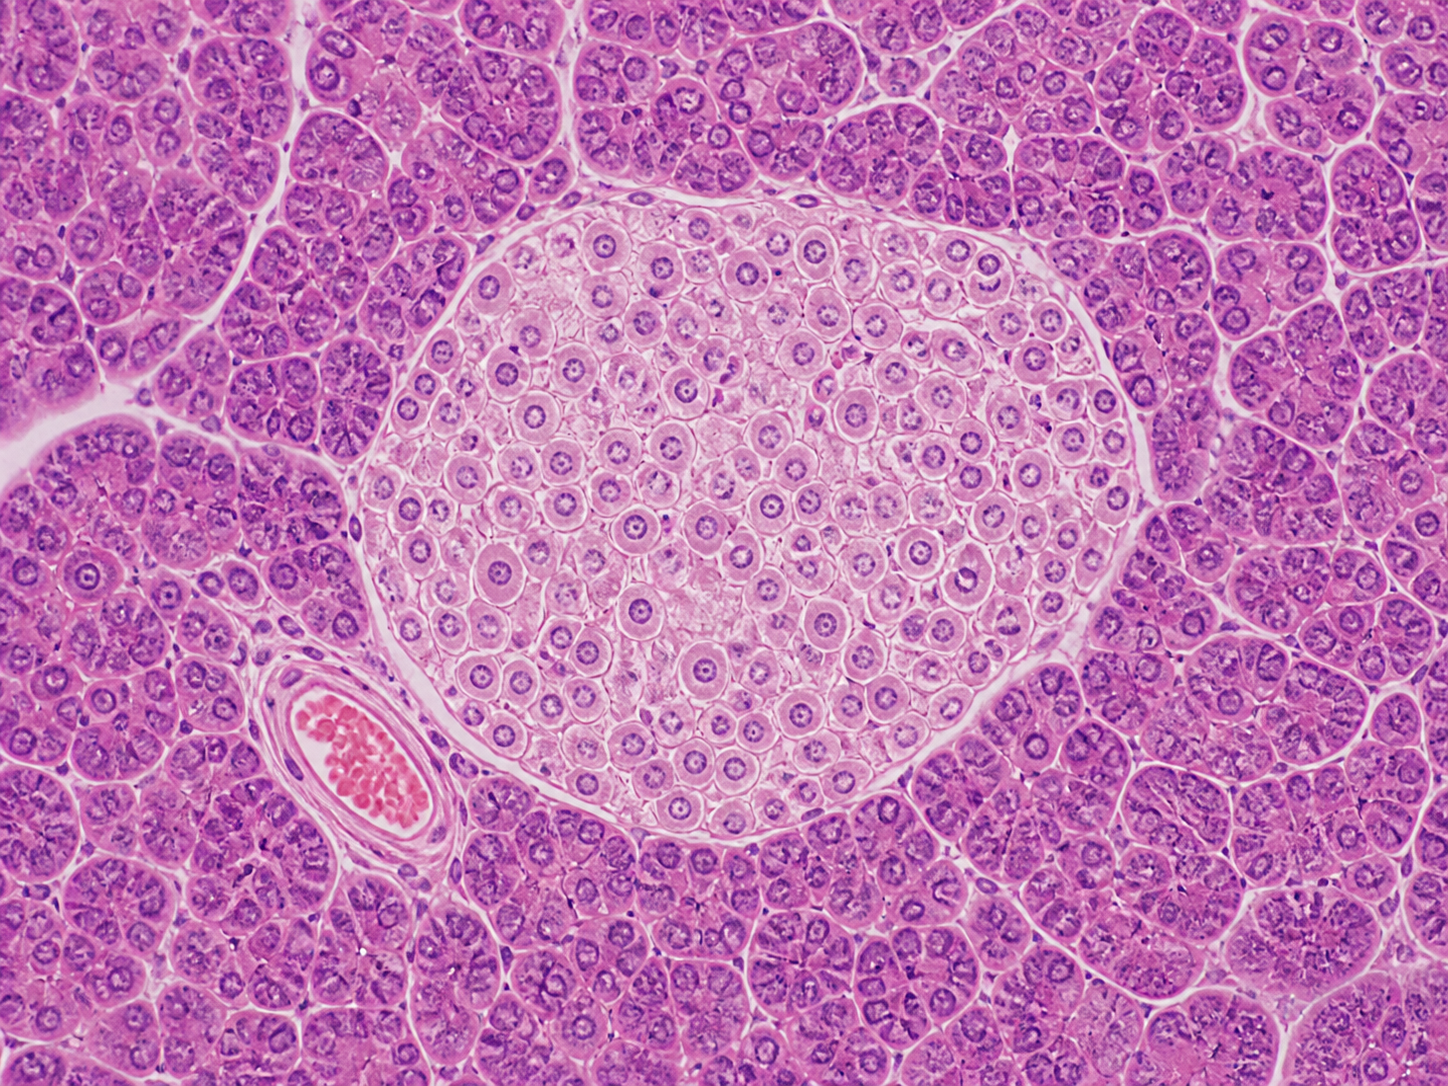
\includegraphics[width=0.56\linewidth]{images/book2/ai/g12-glucose-pancreas-islet.png}

{\small A section of pancreas: an islet, paler, among the darker
clusters of enzyme-secreting \omterm{def:g10:cells-common-unit:cell}{cells}. The islet's \omterm{def:g10:cells-common-unit:cell}{cells} read the blood's
glucose and answer with \omterm{prop:g12:glucose-and-diabetes:hormones}{insulin} or \omterm{prop:g12:glucose-and-diabetes:hormones}{glucagon}; the rest of the organ
makes digestive juice.}
\end{omfigure}

\begin{omfigure}
\begin{tikzpicture}[font=\small, >=Stealth,
  b/.style={draw, rounded corners, align=center, minimum height=1.0cm}]
  \node[b, fill=omThm!15, text width=3.2cm, minimum height=1.4cm] (gly) at (0,0) {glycaemia\\ (set point \qty{1}{g/L})};
  \node[b, fill=omProp!15, text width=2.8cm] (beta) at (-4.6,2.0) {$\beta$ cells: insulin};
  \node[b, fill=omProp!15, text width=2.8cm] (alpha) at (-4.6,-2.0) {$\alpha$ cells: glucagon};
  \node[b, fill=omMeth!15, text width=3.4cm] (store) at (5.6,2.2) {liver, muscle, fat:\\ take up and store glucose};
  \node[b, fill=omMeth!15, text width=3.4cm] (rel) at (5.6,-2.2) {liver: breaks glycogen\\ down, releases glucose};
  \draw[->, thick] (gly.west |- 0,0.4) -- node[above, sloped, font=\scriptsize] {rise detected} (beta.east);
  \draw[->, thick] (gly.west |- 0,-0.4) -- node[below, sloped, font=\scriptsize] {fall detected} (alpha.east);
  \draw[->, thick, omProp] (beta.north) -- ++(0,0.6) -| (store.north);
  \draw[->, thick, omProp] (alpha.south) -- ++(0,-0.6) -| (rel.south);
  \draw[->, thick, omThm] (store.west) -- node[above, sloped, font=\scriptsize, align=center] {glycaemia\\ falls $(-)$} (gly.east |- 0,0.4);
  \draw[->, thick, omThm] (rel.west) -- node[below, sloped, font=\scriptsize, align=center] {glycaemia\\ rises $(+)$} (gly.east |- 0,-0.4);
  \node[font=\scriptsize, anchor=south] at (0,3.3) {insulin};
  \node[font=\scriptsize, anchor=north] at (0,-3.3) {glucagon};
\end{tikzpicture}

{\small The regulation of \omterm{def:g12:glucose-and-diabetes:glycaemia}{glycaemia}. A rise triggers \omterm{prop:g12:glucose-and-diabetes:hormones}{insulin}, which
makes the tissues store glucose and brings the level down; a fall
triggers \omterm{prop:g12:glucose-and-diabetes:hormones}{glucagon}, which makes the liver release glucose and brings
it up. Each \omterm{def:g11:hormones-and-reproduction:hormone}{hormone}'s effect removes the signal that called it: two
negative \omterm{def:g11:hormones-and-reproduction:hormone}{feedback} loops around one set point.}
\end{omfigure}

\begin{example}[The loop in action]\label{ex:g12:glucose-and-diabetes:loop}
After a meal the \omterm{def:g12:glucose-and-diabetes:glycaemia}{glycaemia} climbs; within minutes the $\beta$ \omterm{def:g10:cells-common-unit:cell}{cells}
release \omterm{prop:g12:glucose-and-diabetes:hormones}{insulin}, the muscles and fat \omterm{def:g10:cells-common-unit:cell}{cells} open their glucose
transporters, the liver switches to making \omterm{def:g10:exercise-and-energy:glycogen}{glycogen}, and the level
falls back --- at which point \omterm{prop:g12:glucose-and-diabetes:hormones}{insulin} secretion falls too. Between
meals the drift downward is met by \omterm{prop:g12:glucose-and-diabetes:hormones}{glucagon}, \omterm{def:g10:exercise-and-energy:glycogen}{glycogen} is broken down,
and the level holds. Neither \omterm{def:g11:hormones-and-reproduction:hormone}{hormone} is ever absent; their ratio
moves, and the \omterm{def:g12:glucose-and-diabetes:glycaemia}{glycaemia} follows it within a narrow band.
\end{example}

\section{When the loop fails: diabetes}

\begin{definition}[Diabetes]\label{def:g12:glucose-and-diabetes:diabetes}
\emph{Diabetes}\index{diabetes} is a chronic excess of \omterm{def:g12:glucose-and-diabetes:glycaemia}{glycaemia}:
above \qty{1.26}{g/L} fasting, or above \qty{2}{g/L} two hours after a
standard glucose load. Its early signs follow from the excess: glucose
in the urine, which drags water with it (abundant urine, thirst), and
weight loss when \omterm{def:g10:cells-common-unit:cell}{cells} cannot use the glucose around them. Its late
damage --- to the small vessels of the eye and kidney, to nerves, to
the arteries --- comes from years of glucose reacting with \omterm{def:g11:gene-expression:protein}{proteins}.
Two diseases share the name.
\end{definition}

\begin{proposition}[Type 1 and type 2]\label{prop:g12:glucose-and-diabetes:types}
\begin{itemize}
  \item \emph{Type 1 \omterm{def:g12:glucose-and-diabetes:diabetes}{diabetes}} (about 10\% of cases) is the
        destruction of the $\beta$ \omterm{def:g10:cells-common-unit:cell}{cells} by the patient's own immune
        system, usually in childhood or youth: \omterm{prop:g12:glucose-and-diabetes:hormones}{insulin} is absent. The
        \omterm{def:g12:glucose-and-diabetes:glycaemia}{glycaemia} rises unchecked, fat is burned for lack of usable
        glucose and its acid products accumulate; without injected
        \omterm{prop:g12:glucose-and-diabetes:hormones}{insulin} the disease is fatal within months. Treatment is
        \omterm{prop:g12:glucose-and-diabetes:hormones}{insulin}, several times a day, dosed to the meals and the
        measured \omterm{def:g12:glucose-and-diabetes:glycaemia}{glycaemia}, for life.
  \item \emph{Type 2 \omterm{def:g12:glucose-and-diabetes:diabetes}{diabetes}} (about 90\%) develops in adults, most
        often overweight and inactive: the tissues respond less and
        less to \omterm{prop:g12:glucose-and-diabetes:hormones}{insulin} (\emph{\omterm{prop:g12:glucose-and-diabetes:hormones}{insulin} resistance}), the $\beta$
        \omterm{def:g10:cells-common-unit:cell}{cells} compensate by secreting more, and after years they
        become exhausted. \omterm{prop:g12:glucose-and-diabetes:hormones}{Insulin} is present but insufficient. The
        predisposition is partly genetic
        (\cref{ch:g11:genes-and-disease}); the trigger is the way of
        life, and the first treatment is its change --- weight loss and
        exercise --- before drugs and, late, \omterm{prop:g12:glucose-and-diabetes:hormones}{insulin}.
\end{itemize}
\end{proposition}
\begin{proof}[Evidence]
Type 1 patients have antibodies against their own islet \omterm{def:g10:cells-common-unit:cell}{cells} years
before symptoms, and at diagnosis their \omterm{prop:g12:glucose-and-diabetes:hormones}{islets} are almost empty of
$\beta$ \omterm{def:g10:cells-common-unit:cell}{cells} and infiltrated by white \omterm{def:g10:cells-common-unit:cell}{cells}; their blood \omterm{prop:g12:glucose-and-diabetes:hormones}{insulin} is
undetectable and they respond to injected \omterm{prop:g12:glucose-and-diabetes:hormones}{insulin} at once. Type 2
patients have normal or high \omterm{prop:g12:glucose-and-diabetes:hormones}{insulin} at diagnosis; their muscle and
fat \omterm{def:g10:cells-common-unit:cell}{cells} take up less glucose for a given \omterm{prop:g12:glucose-and-diabetes:hormones}{insulin} dose than a healthy
person's; identical twins share the disease in 70\% of cases, and
weight loss or a walking programme alone restores normal \omterm{def:g12:glucose-and-diabetes:glycaemia}{glycaemia} in
many early cases.
\end{proof}

\begin{omfigure}
\begin{tikzpicture}
\begin{axis}[
  width=0.88\linewidth, height=5.8cm,
  axis x line=bottom, axis y line=left,
  xmin=0, xmax=180, ymin=0, ymax=3,
  xlabel={minutes after drinking \qty{75}{g} of glucose}, ylabel={glycaemia (g/L)},
  xlabel style={font=\small, at={(axis description cs:0.5,-0.12)}, anchor=north},
  ylabel style={font=\small},
  tick label style={font=\small}, xtick={0,30,60,90,120,150,180}, ytick={0,1,2,3},
  legend style={at={(0.5,-0.3)}, anchor=north, legend columns=3, font=\small, draw=none},
  clip=false,
]
\addplot[thick, omMeth, smooth] coordinates {(0,0.9) (30,1.4) (60,1.3) (90,1.1) (120,0.95) (150,0.9) (180,0.9)};
\addplot[thick, omProp, smooth] coordinates {(0,1.1) (30,1.7) (60,1.9) (90,1.85) (120,1.7) (150,1.5) (180,1.35)};
\addplot[thick, omThm, smooth] coordinates {(0,1.6) (30,2.3) (60,2.7) (90,2.8) (120,2.7) (150,2.6) (180,2.5)};
\draw[dashed, gray] (axis cs:0,2) -- (axis cs:180,2);
\node[font=\scriptsize, gray, anchor=south east] at (axis cs:180,2.02) {threshold at 120 min};
\legend{healthy, impaired tolerance, type 2 diabetes}
\end{axis}
\end{tikzpicture}

{\small The glucose tolerance test: \omterm{def:g12:glucose-and-diabetes:glycaemia}{glycaemia} after a standard drink
of \qty{75}{g} of glucose. A healthy person is back near \qty{1}{g/L}
in two hours; a diabetic starts high, climbs above \qty{2}{g/L} and
stays there. The intermediate curve is the warning stage, usually
reversible.}
\end{omfigure}

\begin{example}[Managing a day with type 1]\label{ex:g12:glucose-and-diabetes:type1}
A teenager with type 1 measures her \omterm{def:g12:glucose-and-diabetes:glycaemia}{glycaemia} before each meal with a
drop of blood, counts the \omterm{def:g10:chemistry-of-life:families}{carbohydrate} on her plate, and injects a
dose of fast \omterm{prop:g12:glucose-and-diabetes:hormones}{insulin} proportional to it --- about one unit per
\qty{10}{g} --- plus a slow \omterm{prop:g12:glucose-and-diabetes:hormones}{insulin} once a day for the background. Too
much \omterm{prop:g12:glucose-and-diabetes:hormones}{insulin}, or a missed meal, and the level falls below
\qty{0.6}{g/L}: sweating, trembling, confusion, corrected by sugar in
minutes. Too little, and the level stays above \qty{2}{g/L} with
thirst and fatigue, and the vessels take the damage silently. She is
doing, by hand, what her $\beta$ \omterm{def:g10:cells-common-unit:cell}{cells} did by \omterm{def:g11:hormones-and-reproduction:hormone}{feedback}.
\end{example}

\begin{omfigure}
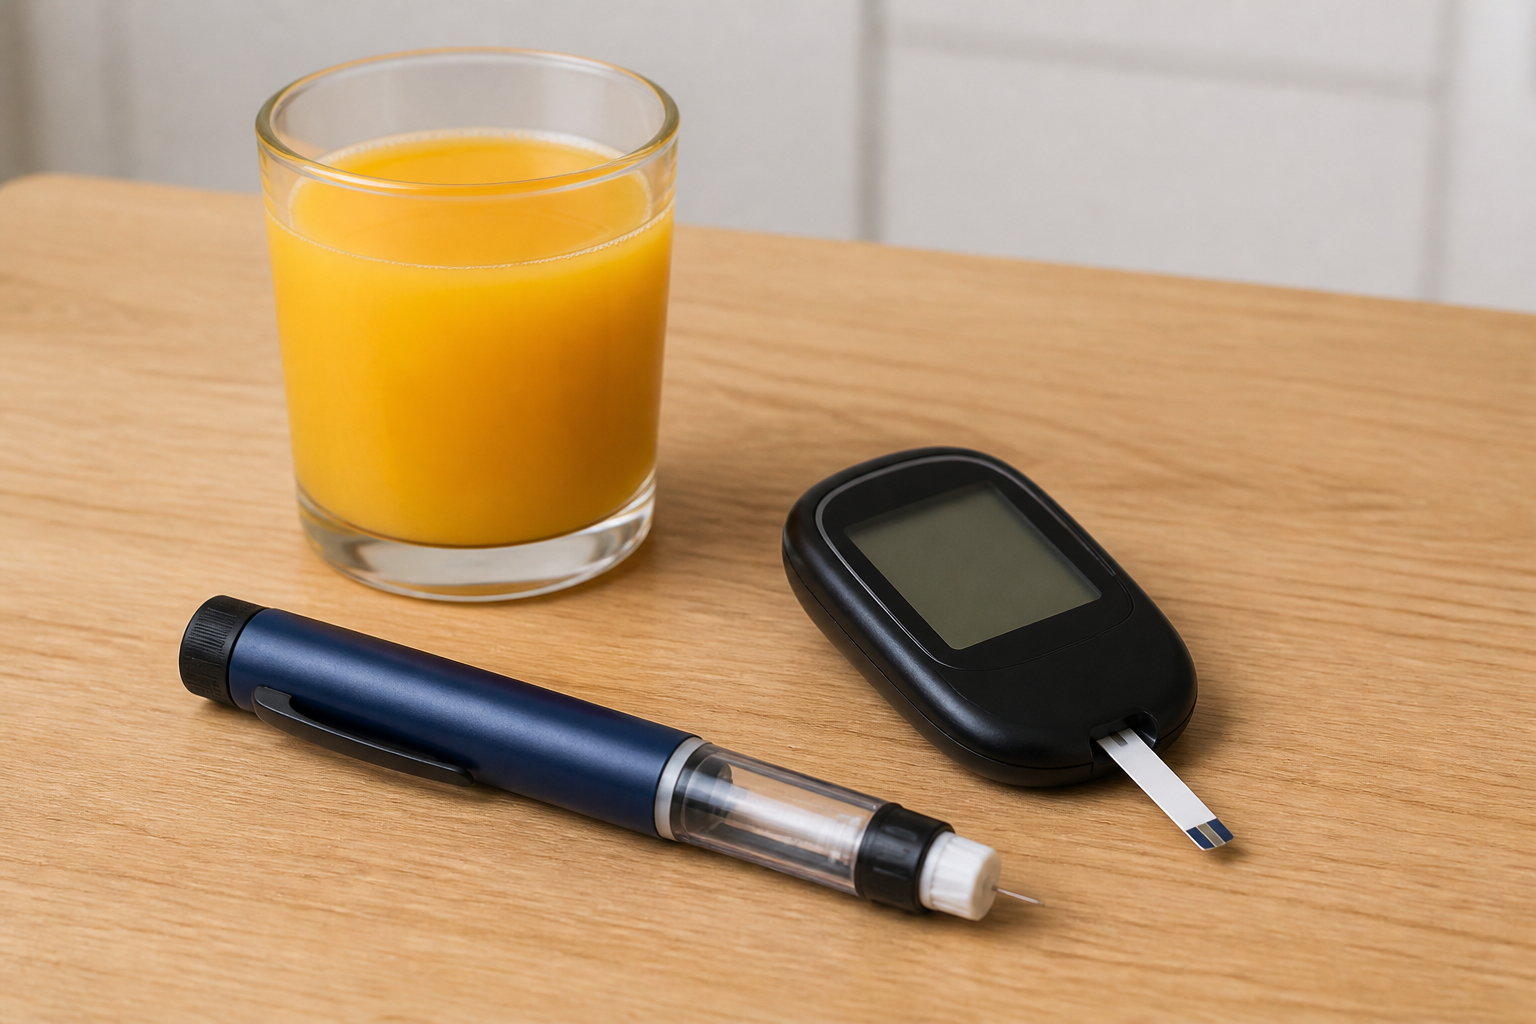
\includegraphics[width=0.56\linewidth]{images/book2/ai/g12-glucose-meter-pen.png}

{\small The tools of a type 1 diabetic: a meter that reads the
\omterm{def:g12:glucose-and-diabetes:glycaemia}{glycaemia} from a drop of blood, and a pen that injects a measured dose
of \omterm{prop:g12:glucose-and-diabetes:hormones}{insulin}. The loop of the \omterm{prop:g12:glucose-and-diabetes:hormones}{islets}, run by hand several times a day.}
\end{omfigure}

\begin{method}[Reading a glycaemia record]\label{met:g12:glucose-and-diabetes:read}
\begin{enumerate}
  \item Locate the set point and the band: fasting \qtyrange{0.7}{1.1}{g/L},
        after meals below \num{1.4}; two hours after a glucose load
        below \num{1.4} (healthy), \qtyrange{1.4}{2}{} (impaired),
        above \qty{2}{g/L} (\omterm{def:g12:glucose-and-diabetes:diabetes}{diabetes}).
  \item For each rise, ask what put glucose in (meal, liver) and what
        should take it out (\omterm{prop:g12:glucose-and-diabetes:hormones}{insulin}'s targets); for each fall, what
        took it out (brain, muscle) and what should put it back
        (\omterm{prop:g12:glucose-and-diabetes:hormones}{glucagon}, the liver).
  \item Read the \omterm{def:g11:hormones-and-reproduction:hormone}{hormones} with the glucose: \omterm{prop:g12:glucose-and-diabetes:hormones}{insulin} should rise with
        the \omterm{def:g12:glucose-and-diabetes:glycaemia}{glycaemia} and \omterm{prop:g12:glucose-and-diabetes:hormones}{glucagon} fall; absent \omterm{prop:g12:glucose-and-diabetes:hormones}{insulin} means type 1,
        high \omterm{prop:g12:glucose-and-diabetes:hormones}{insulin} with high \omterm{def:g12:glucose-and-diabetes:glycaemia}{glycaemia} means resistance.
  \item Convert units when needed: \qty{1}{g/L} of glucose is
        \qty{5.55}{mmol/L}.
\end{enumerate}
\end{method}

\begin{remark}[A model of regulation]\label{rem:g12:glucose-and-diabetes:model}
Sensor, set point, two opposed effectors, negative \omterm{def:g11:hormones-and-reproduction:hormone}{feedback}: the
control of \omterm{def:g12:glucose-and-diabetes:glycaemia}{glycaemia} is the same design as the control of testosterone
in \cref{ch:g11:hormones-and-reproduction}, and the design of most of
the body's constants --- temperature, water, blood pressure, acidity.
\omterm{def:g12:glucose-and-diabetes:diabetes}{Diabetes} is what a regulated constant looks like when its loop is
broken: the value still responds to inputs, but nothing brings it back.
Reading the curves of this chapter is practice for reading any of
them.
\end{remark}

\section{Exercises}

\begin{exercise}[$\star$]\label{exo:g12:glucose-and-diabetes:1}
Give the normal fasting \omterm{def:g12:glucose-and-diabetes:glycaemia}{glycaemia} in \unit{g/L} and in \unit{mmol/L},
and the two danger thresholds.
\end{exercise}

\begin{exercise}[$\star$]\label{exo:g12:glucose-and-diabetes:2}
Name the two \omterm{def:g11:hormones-and-reproduction:hormone}{hormones} of the \omterm{prop:g12:glucose-and-diabetes:hormones}{islets}, the \omterm{def:g10:cells-common-unit:cell}{cells} that make them, and the
effect of each on the \omterm{def:g12:glucose-and-diabetes:glycaemia}{glycaemia}.
\end{exercise}

\begin{exercise}[$\star$]\label{exo:g12:glucose-and-diabetes:3}
Which organ can both store and release glucose? In what form does it
store it?
\end{exercise}

\begin{exercise}[$\star$]\label{exo:g12:glucose-and-diabetes:4}
State the essential difference between type 1 and type 2 \omterm{def:g12:glucose-and-diabetes:diabetes}{diabetes} in
one sentence each.
\end{exercise}

\begin{exercise}[$\star$]\label{exo:g12:glucose-and-diabetes:5}
From the tolerance-test figure, read the three curves at 120 minutes
and classify each.
\end{exercise}

\begin{exercise}[$\star\star$]\label{exo:g12:glucose-and-diabetes:6}
The brain uses \qty{5}{g} of glucose per hour and the blood holds
\qty{5}{g}. Explain why a person does not lose consciousness an hour
after a meal, naming the organ and the \omterm{def:g11:hormones-and-reproduction:hormone}{hormone} responsible.
\end{exercise}

\begin{exercise}[$\star\star$]\label{exo:g12:glucose-and-diabetes:7}
Explain why removing the pancreas causes \omterm{def:g12:glucose-and-diabetes:diabetes}{diabetes} but tying its duct
does not, and what this shows about where \omterm{prop:g12:glucose-and-diabetes:hormones}{insulin} is made and how it
travels.
\end{exercise}

\begin{exercise}[$\star\star$]\label{exo:g12:glucose-and-diabetes:8}
A fasting person receives an injection of \omterm{prop:g12:glucose-and-diabetes:hormones}{glucagon}: the \omterm{def:g12:glucose-and-diabetes:glycaemia}{glycaemia}
rises by \qty{0.4}{g/L} in 20 minutes. The same injection after three
days of fasting does nothing. Explain.
\end{exercise}

\begin{exercise}[$\star\star$]\label{exo:g12:glucose-and-diabetes:9}
Why does a diabetic pass abundant urine and feel thirsty?
\end{exercise}

\begin{exercise}[$\star\star$]\label{exo:g12:glucose-and-diabetes:10}
A type 1 patient injects her usual dose of \omterm{prop:g12:glucose-and-diabetes:hormones}{insulin} and then skips
lunch. Predict what happens over the next two hours and why.
\end{exercise}

\begin{exercise}[$\star\star$]\label{exo:g12:glucose-and-diabetes:11}
Explain why exercise lowers the \omterm{def:g12:glucose-and-diabetes:glycaemia}{glycaemia} of a type 2 diabetic even
without any change in \omterm{prop:g12:glucose-and-diabetes:hormones}{insulin}, using \cref{ch:g10:sport-and-health}.
\end{exercise}

\begin{exercise}[$\star\star\star$]\label{exo:g12:glucose-and-diabetes:12}
Two patients have a fasting \omterm{def:g12:glucose-and-diabetes:glycaemia}{glycaemia} of \qty{2}{g/L}. One has no
detectable \omterm{prop:g12:glucose-and-diabetes:hormones}{insulin}; the other has three times the normal \omterm{prop:g12:glucose-and-diabetes:hormones}{insulin}.
Diagnose each, and say what each patient's \omterm{prop:g12:glucose-and-diabetes:hormones}{islets} are doing.
\end{exercise}

\begin{exercise}[$\star\star\star$]\label{exo:g12:glucose-and-diabetes:13}
Draw, or describe, the curves of \omterm{def:g12:glucose-and-diabetes:glycaemia}{glycaemia} and of \omterm{prop:g12:glucose-and-diabetes:hormones}{insulin} over the
three hours after a meal in a healthy person, in a type 1 patient
without treatment, and in a type 2 patient. Explain each difference.
\end{exercise}

\begin{exercise}[$\star\star\star$]\label{exo:g12:glucose-and-diabetes:14}
A meal contains \qty{80}{g} of \omterm{def:g10:chemistry-of-life:families}{carbohydrate}. If all of it entered the
blood at once, what would the \omterm{def:g12:glucose-and-diabetes:glycaemia}{glycaemia} become? Explain why it never
does, listing the fates of the glucose in the first two hours.
\end{exercise}

\begin{exercise}[$\star\star\star$]\label{exo:g12:glucose-and-diabetes:15}
Compare the regulation of \omterm{def:g12:glucose-and-diabetes:glycaemia}{glycaemia} with that of testosterone in
\cref{ch:g11:hormones-and-reproduction}: sensor, set point,
effectors, sign of the \omterm{def:g11:hormones-and-reproduction:hormone}{feedback}. What is special about having two
opposed \omterm{def:g11:hormones-and-reproduction:hormone}{hormones}?
\end{exercise}

\section{Problem: Five Grams of Sugar}

\begin{problem}[{Weekend problem --- the glucose of the blood
accounted for over a day: the pool and its flows, a tolerance test
read, an insulin dose computed, and a loop that has to be replaced by
hand}]
\label{pb:g12:glucose-and-diabetes:1}
Take a blood volume of \qty{5}{L}, a brain consumption of
\qty{5}{g/h} of glucose, a liver \omterm{def:g10:exercise-and-energy:glycogen}{glycogen} store of \qty{100}{g}, and
muscle \omterm{def:g10:exercise-and-energy:glycogen}{glycogen} of \qty{400}{g}. One unit of fast \omterm{prop:g12:glucose-and-diabetes:hormones}{insulin} disposes of
about \qty{10}{g} of \omterm{def:g10:chemistry-of-life:families}{carbohydrate}.

\medskip
\noindent\textbf{Part I --- The pool.}
\begin{enumerate}
  \item Compute the mass of glucose in the blood at \qty{1}{g/L}, and
        the same concentration in \unit{mmol/L} (glucose
        \qty{180}{g/mol}).
  \item How long would the blood's glucose last the brain alone, if
        nothing replaced it?
  \item Between meals, the liver replaces it. How long does the
        liver's \omterm{def:g10:exercise-and-energy:glycogen}{glycogen} last the brain? What happens after that?
  \item Muscle \omterm{def:g10:exercise-and-energy:glycogen}{glycogen} is four times the liver's, but muscles cannot
        release glucose into the blood. Explain why muscle \omterm{def:g10:exercise-and-energy:glycogen}{glycogen}
        does not help the brain, and what it is for.
  \item A meal delivers \qty{60}{g} of glucose over an hour. If none
        were removed, what would the \omterm{def:g12:glucose-and-diabetes:glycaemia}{glycaemia} reach? What actually
        removes it, and where does it go?
\end{enumerate}

\medskip
\noindent\textbf{Part II --- The test.}
A patient drinks \qty{75}{g} of glucose. Measured \omterm{def:g12:glucose-and-diabetes:glycaemia}{glycaemia} and
\omterm{prop:g12:glucose-and-diabetes:hormones}{insulin}:

\begin{center}
\begin{tabular}{lcccccc}
minutes & 0 & 30 & 60 & 90 & 120 & 180 \\ \hline
\omterm{def:g12:glucose-and-diabetes:glycaemia}{glycaemia} (g/L) & 1.15 & 1.8 & 2.05 & 2.0 & 1.85 & 1.6 \\
\omterm{prop:g12:glucose-and-diabetes:hormones}{insulin} (\% of a healthy peak) & 90 & 140 & 180 & 200 & 190 & 160 \\
\end{tabular}
\end{center}
\begin{enumerate}[resume]
  \item Classify the patient with the thresholds of
        \cref{met:g12:glucose-and-diabetes:read}.
  \item Is \omterm{prop:g12:glucose-and-diabetes:hormones}{insulin} lacking? What, then, is failing?
  \item Name the disease, and give two features of the patient's
        history you would expect.
  \item What would the same table look like for a type 1 patient
        without treatment?
  \item What is the first treatment prescribed, and by what
        mechanism does it act?
\end{enumerate}

\medskip
\noindent\textbf{Part III --- Running the loop by hand.}
A type 1 patient's \omterm{def:g12:glucose-and-diabetes:glycaemia}{glycaemia} is \qty{1.0}{g/L} before dinner; the meal
holds \qty{90}{g} of \omterm{def:g10:chemistry-of-life:families}{carbohydrate}.
\begin{enumerate}[resume]
  \item Compute the dose of fast \omterm{prop:g12:glucose-and-diabetes:hormones}{insulin} for the meal.
  \item She injects it but eats only half the meal. Estimate how far
        the \omterm{def:g12:glucose-and-diabetes:glycaemia}{glycaemia} may fall, and name the symptoms and the remedy.
  \item She injects nothing and eats the whole meal. Estimate the
        \omterm{def:g12:glucose-and-diabetes:glycaemia}{glycaemia} if the \qty{90}{g} all entered a \qty{5}{L} pool, and
        say what the kidneys do above \qty{1.8}{g/L}.
  \item Why must she also inject a slow \omterm{prop:g12:glucose-and-diabetes:hormones}{insulin} at night, when she
        eats nothing?
  \item Explain in what sense the meter and the pen replace the
        $\beta$ \omterm{def:g10:cells-common-unit:cell}{cell}, and what they cannot replace.
\end{enumerate}

\medskip
\noindent\textbf{Part IV --- The loop, reasoned.}
\begin{enumerate}[resume]
  \item A drug stimulates the $\beta$ \omterm{def:g10:cells-common-unit:cell}{cells} to secrete more \omterm{prop:g12:glucose-and-diabetes:hormones}{insulin}.
        For which type of \omterm{def:g12:glucose-and-diabetes:diabetes}{diabetes} can it work, and why not for the
        other?
  \item A person with type 2 loses \qty{10}{kg} and walks an hour a
        day; six months later the tolerance test is normal. Explain
        which part of the loop was repaired.
  \item Explain why a healthy person's \omterm{prop:g12:glucose-and-diabetes:hormones}{insulin} and \omterm{prop:g12:glucose-and-diabetes:hormones}{glucagon} are never
        both high, and what an islet in a dish does when the glucose
        of the medium is set at \qty{1}{g/L}.
  \item \omterm{prop:g12:glucose-and-diabetes:hormones}{Glucagon}, \omterm{prop:g10:heart-lungs-effort:control}{adrenaline}, cortisol and growth \omterm{def:g11:hormones-and-reproduction:hormone}{hormone} all raise
        the \omterm{def:g12:glucose-and-diabetes:glycaemia}{glycaemia}; only \omterm{prop:g12:glucose-and-diabetes:hormones}{insulin} lowers it. Propose why the body
        has several safeguards against a low \omterm{def:g12:glucose-and-diabetes:glycaemia}{glycaemia} and one against
        a high one.
  \item State the result: the glucose in the blood, the hours the
        liver can cover, the diagnosis of Part II, and the dose of
        Part III.
\end{enumerate}
\end{problem}
